%!TEX root = ../../paper.tex

\begin{figure}
	\centering
	\beforeFinalVersion{Remove ticks and labels.}
	%!TEX root = ../../paper.tex

% Ferdosi Set 2
\begin{subfigure}{0.23\textwidth}
	\centering
	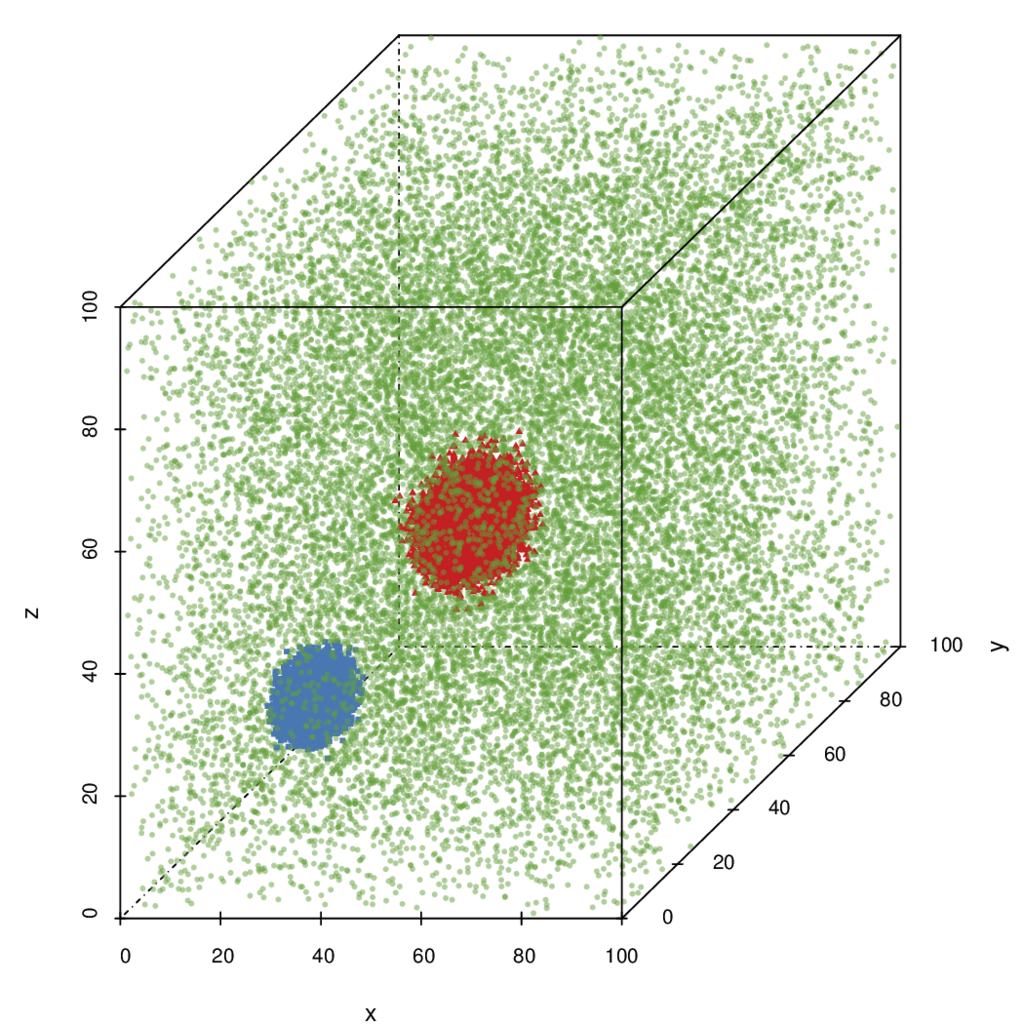
\includegraphics[width=\textwidth]{experiment/img/datasetplot_ferdosi_2_60000}
	\caption{Set \ferdosiTwo}
	\label{fig:experiment:multisphere:ferdosi2}
\end{subfigure}	
% Ferdosi Set 3
\begin{subfigure}{0.23\textwidth}
	\centering
	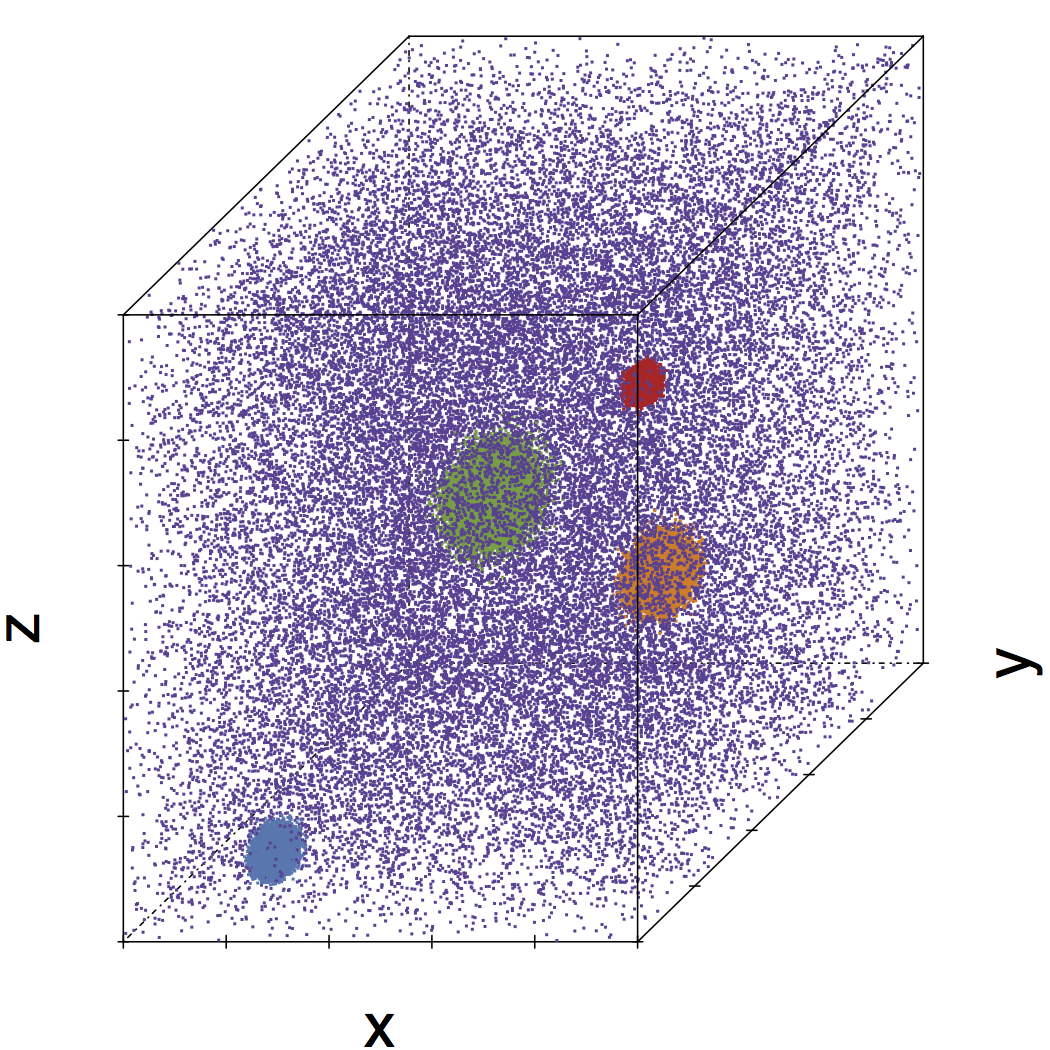
\includegraphics[width=\textwidth]{experiment/img/datasetplot_ferdosi_3_120000}
	\caption{Set \ferdosiThree}
	\label{fig:experiment:multisphere:ferdosi3}
\end{subfigure}	
\subfigvspace
% Baakman 2
\begin{subfigure}{0.23\textwidth}
	\centering
	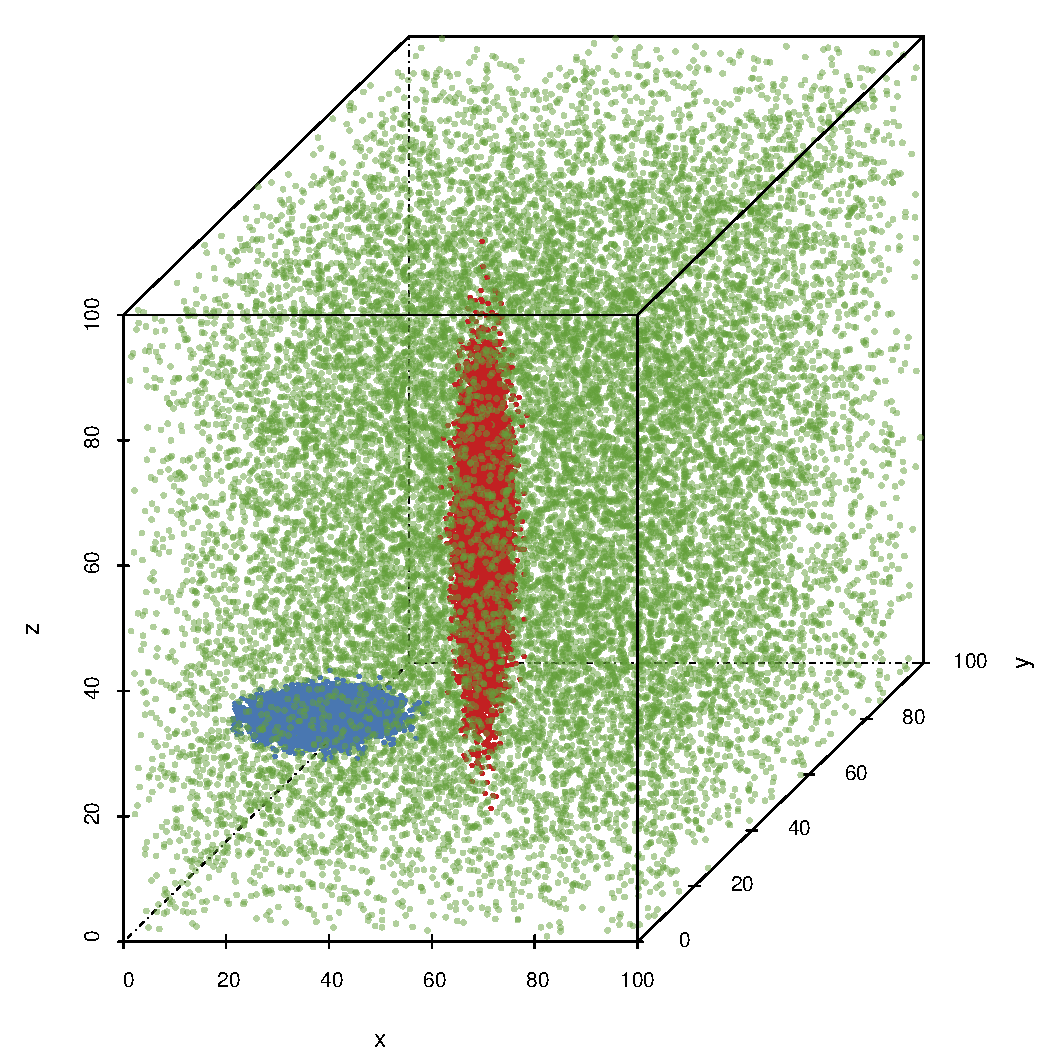
\includegraphics[width=\textwidth]{experiment/img/datasetplot_baakman_2_60000}
	\caption{Set \baakmanTwo}
	\label{fig:experiment:multisphere:baakman2}
\end{subfigure}			
% Baakman 3
\begin{subfigure}{0.23\textwidth}
	\centering
	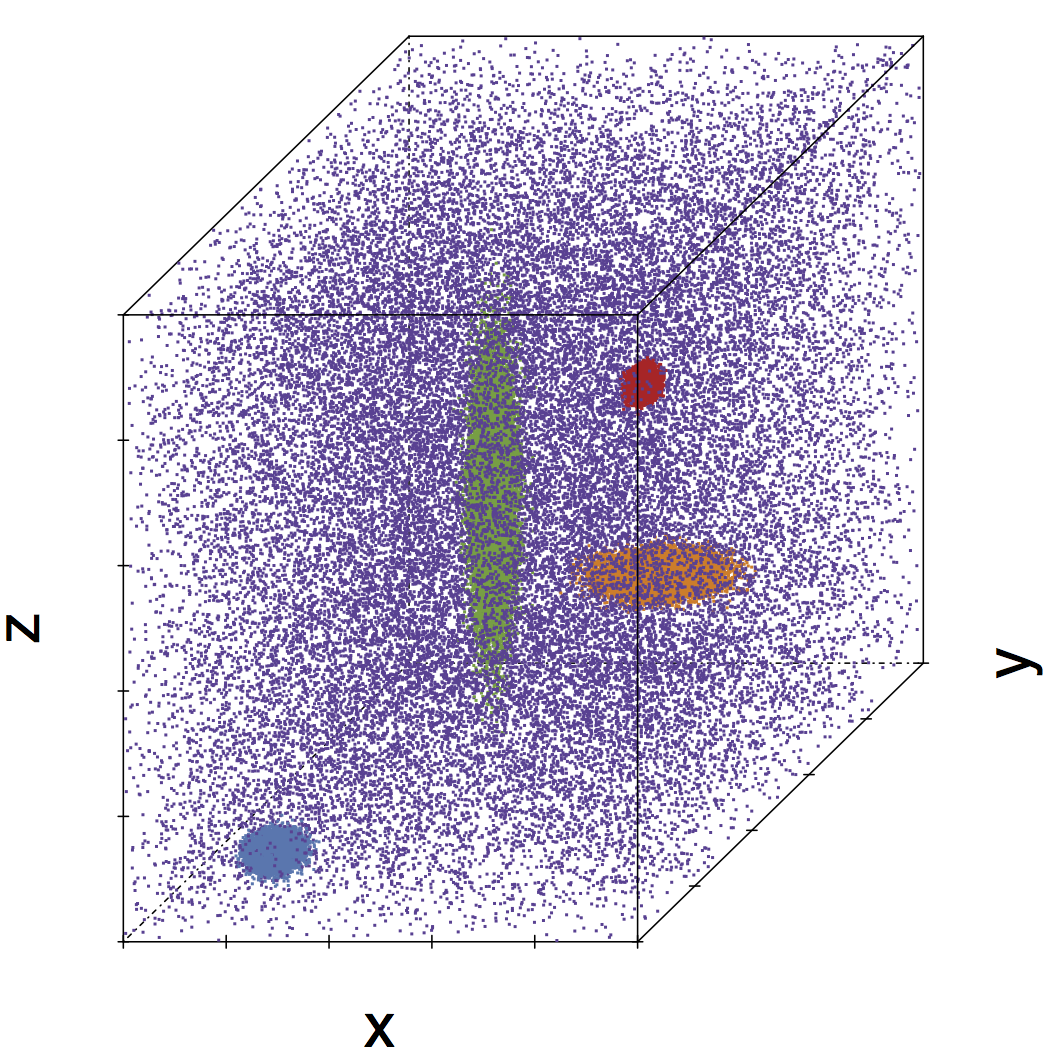
\includegraphics[width=\textwidth]{experiment/img/datasetplot_baakman_3_120000}
	\caption{Set \baakmanThree}
	\label{fig:experiment:multisphere:baakman3}
\end{subfigure}
	\caption{Scatter plot representation of the datasets defined in \cref{tab:experiment:multisphere:sets}, the colors used for the different components correspond to those in \cref{tab:experiment:multisphere:sets}.}
	\label{fig:experiment:multisphere:sets}
\end{figure}

\begin{table*}
	\centering
	%!TEX root = ../../paper.tex
\small
\sisetup{
	table-format=5.0,
	scientific-notation=false,
	round-mode=places,
	round-precision=1,
	table-number-alignment=center
}
\begin{tabular}{@{}cclSl@{}}
\toprule
				&~						& Component					& {Samples} 	& Distribution\\
\midrule
% Ferdosi 1
\ferdosiOne 	&\legendComponentOne	& Trivariate Gaussian 		& 40000		& $\gaussDist{[50, 50, 50]}{\diag(11)}$\\
~ 				&\legendComponentNoise	& Uniform random background	& 20000		& $\uniformDist{[0, 0, 0]}{[100, 100, 100]}$\\
% Baakman 1
\hline
\baakmanOne		&\legendComponentOne	& Trivariate Gaussian 		& 40000		& $\gaussDist{[50, 50, 50]}{\diag([11^2, \sqrt{11}, \sqrt{11}])}$\\
~ 				&\legendComponentNoise	& Uniform random background	& 20000		& $\uniformDist{[0, 0, 0]}{[100, 100, 100]}$\\
% Baakman 4
\hline
\baakmanFour	&\legendComponentOne	& Trivariate Gaussian 		& 40000		& $\gaussDist{[50, 50, 50]}{\diag([11, 2 * \sqrt{11}, \rfrac{1}{2} \sqrt{11}])}$\\
~ 				&\legendComponentNoise	& Uniform random background	& 20000		& $\uniformDist{[0, 0, 0]}{[100, 100, 100]}$\\
% Baakman 5
\hline
\baakmanFive	&\legendComponentOne	& Trivariate Gaussian 		& 40000		& $\gaussDist{[50, 50, 50]}{\diag([11^2, 11, 1])}$\\
~ 				&\legendComponentNoise	& Uniform random background	& 20000		& $\uniformDist{[0, 0, 0]}{[100, 100, 100]}$\\
\bottomrule
\end{tabular}
	\caption{The datasets with multiple Gaussian distributions embedded in uniform noise. This table has the same structure and uses the same notation as \cref{tab:experiment:singlesphere:sets}.} 	
	\label{tab:experiment:multisphere:sets}
\end{table*}

%General
\Cref{tab:experiment:multisphere:sets} defines the datasets that consist of uniform random noise and multiple Gaussian distributions, a scatter plot representation of these sets is shown in \cref{fig:experiment:multisphere:sets}. 
	% Ferdosi 2
	Dataset \ferdosiTwo consists of two Gaussian distributions, that are unlikely to overlap, embedded in noise. The first Gaussian component is significantly denser than the second. 
	% Baakman 2
	The procedure outlined in \cref{s:experiment:singlesphere} for the creation of dataset \baakmanOne was used to derive dataset \baakmanTwo from \ferdosiTwo.
	% Ferdosi Three
	Dataset \ferdosiThree embeds four non-overlapping Gaussians, with eigenspheres with notably different radii, in the uniform random background. 
	%Baakman 3
	The last dataset, \baakmanThree, is a variation on \ferdosiThree, created with the method that was used for the definition of dataset \baakmanOne from \ferdosiOne. 

%Hypothesis
	Due to the spherical nature of the Gaussian components we expect hardly any difference in performance between the estimators on dataset \ferdosiTwo and \ferdosiThree. Given the shape of the Gaussian distributions embedded in dataset \baakmanTwo and \baakmanThree we hypothesize that \sambe outperforms \mbe on these sets.